\documentclass{scrartcl}

\usepackage[utf8]{inputenc}
\usepackage[T1]{fontenc}
\usepackage{lmodern}
\usepackage[ngerman]{babel}
\usepackage{amsmath}
\usepackage{hyperref}
\usepackage{pdfpages}

\title{Dokumentation Softwareprojekt}

\date{19. Juni 2016}
\begin{document}

\maketitle
\tableofcontents
\newpage

\section{Einleitung}

Diese Dokumentation behandelt unsere Vorgehensweise beim Softwareprojekt...

\subsection{Projektbeschreibung}

Im Rahmen der Veranstaltung mussten wir uns, für die Bearbeitung von Softwareprojekten in Gruppen zusammenfinden. Anschließend musste sich jedes Team eine/n betreuende/n Professor/in suchen und mit dieser/m ein Projekt, zur Umsetzung innerhalb von 2 Semestern, planen und durchführen. Unser Team, bestehend aus Edgar Filipsen, Mika Katzwinkel, Jakob Kost, Hubert Richter und Sebastian Schreiter suchte sich Frau Prof. Dr. rer. nat. Brabender als betreuende Professorin aus. 

\section{Eingesetzte Tools/Werkzeuge}

\subsection{ROS Indigo}

\subsection{RViz}

\section{Eingesetzte Hardware}

\subsection{NAO Roboter}

\subsection{Minigolf Ausrüstung}

\subsubsection{Die Bahn}
Da der neue NAO Schwierigkeiten mit dem Teppichboden unseres Büros hatte und um gleichbleibende Bedingungen zu ermöglichen, entschieden wir uns für eine Bahn aus Holz mit den Maßen: 2,5m x 1,35m. Bis auf den Startbereich ist die Bahn von einem 5cm hohen Rand umgeben, welcher als Bande dienen soll. Das Ziel hat einen Durchmesser von 15cm und ist 45cm vom hinteren Rand entfernt (siehe Anhang A1). Zudem entschieden wir uns für zwei kreisrunde Hindernisse in blau und grün mit einem Durchmesser von 18cm. Um  optimale Voraussetzungen für die Erkennung des Balls, sowie der Hindernisse zu ermöglichen wurde die Bahn weiß.

\subsubsection{Der Schläger}

\subsubsection{Der Ball}
Wir testeten über Monate verschiedene Bälle, sowohl in Hinblick auf Größe als auch auf Material. Die Wahl der Farbe fiel direkt auf rot, da der NAO bereits eine RedBall Detection besitzt

\section{Ablauf}



\section{Installation}


\subsection{Installation von ROS}

Für das Projekt entschieden wir uns für ROS Indigo, die aktuellste Version mit Langzeitunterstützung.
Die Installation erfolgte auf Ubuntu 14.04 
Als Grundlage nutzten wir das offizielle Installationstutorial des ROS Wikis.
Zunächst mussten Pakete von packages.ros.org akzeptiert werden. Der Befehl dazu lautet: 
\begin{align}
&sudo\ sh\ -c\ 'echo\ ``deb\ http://packages.ros.org/ros/ubuntu \\ 
&\$(lsb\_release\ -sc)\ main"\ >\ /etc/apt/sources.list.d/ros-latest.list'
\end{align}
Außerdem muss noch die Schlüssel ID  zur Authentifizierung der Pakete vom Server heruntergeladen werden:
\begin{align}
&sudo\ apt-key\ adv\ --keyserver\ hkp://ha.pool.sks-keyservers.net\\ 
& --recv-key\ 0xB01FA116
\end{align}
Mit dem Befehl 
\begin{align}
&sudo\ apt-get\ install\ ros-indigo-desktop-full
\end{align}
wird die komplette Installation gestartet, die folgende Komponenten enthält: ROS, rqt, rviz, robot-generic libraries, 2D/3D Simulatoren, Navigation und Pakete für die 2D und 3D Wahrnehmung.
\\
Bevor ROS nun genutzt werden kann, muss rosdep initialisiert werden. Dies erlaubt die einfache Eingabe von...
\begin{align}
&sudo\ rosdep\ init\\
&rosdep\ update
\end{align}
Um die setup.bash Datei nicht bei jedem Öffnen einer neuen Shell sourcen zu müssen, empfiehlt es sich, diesen Befehl in die .bashrc-Datei zu kopieren.
Dafür nutzten wir folgende Befehle:
\begin{align}
&echo\ ``source\ /opt/ros/indigo/setup.bash"\ >>\ \sim/.bashrc\\
&source\ \sim/.bashrc
\end{align}

\subsection{Erstellen von Workspace}

Nach der Installation ist es nötig, einen Workspace zu erstellen, in dem gearbeitet wird.

\begin{align}
&\$\ mkdir\ -p\ \sim/catkin\_ws/src\\
&\$\ cd\ \sim/catkin\_ws/src\\
&\$\ catkin\_init\_workspace
\end{align}

\subsection{Tutorial}

Auf der ROS-Wikiseite http://wiki.ros.org/ROS/Tutorials finden sich viele Tutorials, welche den Umgang mit dem ROS Filesystem, Packages und Nodes, sowie das Schreiben von Publishern und Subscribern in C++ oder Python beschreiben.
Diese wurden von uns zur Einarbeitung bearbeitet.

\subsection{Installation von RVIZ}

Die Installation von RViz war bereits im Installationspaket von ROS enthalten und musste hierfür nicht noch einmal gesondert installiert werden. Allerdings musste noch zusätzlich das ganze NAO-Paket, wie z.B. Treiber u.Ä. installiert werden. Über die Seite http://wiki.ros.org/nao/Tutorials/Installation gelangt man zu einem Tutorial, in dem alles Nötige erklärt wird. Nachdem wir dieses Tutorial durchgearbeitet hatten, war die Installation aller wichtigen Komponenten fast fertiggestellt. Um ein schon fertiges Modell des NAO-Roboters benutzen zu können, mussten wir noch ein zusätzliches Paket herunterladen und dazu einer Lizenzbestimmung zustimmen. Dieses wird über den Befehl
\begin{align}
&sudo\ apt-get\ install\ ros-indigo-nao-meshes
\end{align}
heruntergeladen und installiert.

\subsection{Konfiguration von RVIZ für den NAO}

Bei der Konfiguration von ROS für den NAO-Roboter sahen wir uns einigen Problemen gegenübergestellt. Zunächst war das Tutorial, welches auf der ROS-Wikiseite zu finden ist, veraltet. Das Problem dabei war, dass dieses das einzige Tutorial war, das wir auffinden konnten. Deshalb mussten wir uns erst einmal eine ganze Weile mit RViz auseinander setzen. Nach dem Durchforsten einiger Foreneinträge und auch ein wenig Ausprobieren, fanden wir dann die richtigen Befehle, um eine ordentliche Simulation des NAO über RViz laufen zu lassen.
Zunächst wird der Roscore gestartet:
\begin{align}
&cd\ \sim/catkin\_ws\\
&roscore
\end{align}
Anschließend werden die Simulation und die dazugehörigen Treiber gestartet:
\begin{align}
&\sim/naoqi/naoqi\-sdk\-2.1.4.13\-linux64/naoqi\ --verbose\ \-\-broker-ip\ 127.0.0.1\\
&roslaunch\ naoqi\_driver\_py\ naoqi\_driver.launch
\end{align}
Für den letzten Schritt bearbeiteten wir eine bereits vorhandene .launch-Datei so, dass RViz nach unseren Vorstellungen das Modell lädt. Das ganze startet man dann über folgenden Befehl:
\begin{align}
&roslaunch\ nao\_description\ display.launch
\end{align}
display.launch ist hierbei unsere editierte Datei.
Damit haben wir einen simulierten NAO-Roboter, dem wir per Konsole Befehle erteilen können.

\subsection{Einarbeitung in NAO-API}

Nachdem wir dem NAO-Roboter ein paar Befehle direkt über die Konsole erteilt hatten, ging es nun darum, ihn komplexere Befehlssätze ausführen zu lassen. 
Dazu mussten wir uns allerdings zunächst in die NAO-API einarbeiten, welche unter folgender Adresse zu erreichen ist:\\
\url{http://doc.aldebaran.com/1-14/naoqi/index.html} \\
Zusätzlich dazu schauten wir uns auch einige Code-Beispiele zu wichtigen Themen, wie z.B. der Ballerkennung an, um die Funktionsweise der einzelnen Befehle zu verstehen.


\section{Programmierung}


\subsection{Erste Schritte}

Nachdem wir die Installation und Konfiguration durchgeführt hatten, testeten wir zunächst einige Grundfunktionen anhand der Visualisierung mit RViz.
Hierbei nutzten wir die Konsole um Befehle direkt zu übermitteln. Dabei stellten wir fest, dass einige Befehle in der Visualisierung nicht umgesetzt werden konnten, da das genutzte Modell in RViz nicht vollständig war.
Im Anschluss führten wir die Kommandos am Roboter aus, was weniger Probleme verursachte, als wir uns vorgestellt hatten. 
Dennoch mussten wir uns noch viel mit der NAO-API auseinander setzen, um die benötigten Schnittstellen zu finden.

\subsection{Schlagbewegung}

Um die Schlagbewegung durchzuführen testeten wir zunächst die ungefähren Bewegungen in der Simulation. Am Roboter führten wir danach die Feinabstimmung durch und nutzten dabei einen kleinen Spielzeuggolfschläger. 
Da sich in diesem Abschnitt herausstellte, dass das Ausführen unter ROS sehr viel Zeit beanspruchte, verzichteten wir im Folgenden temporär auf ROS und nutzten stattdessen einfache Python-Skripte, um Änderungen schneller austesten zu können.

\subsection{Ballerkennung}

Da der NAO bereits eine Funktion für die Erkennung eines roten Balls besitzt, nutzten wir diese direkt. Hierfür besorgten wir uns einen roten Plastikball und führten erste Versuche durch, um die Funktion für unsere Zwecke einsetzen zu können.
Allerdings mussten wir hierbei einige Anpassungen vornehmen, weil die Kamera des NAO nur einen bestimmten Sichtbereich hat und der Bereich direkt vor dem Roboter nicht mehr sichtbar ist. Da wir deshalb das letzte Stück ''blind'' steuern mussten, kam es hierbei auch häufig zu Ungenauigkeiten beim Schlag. Daraus resultierte eine schwer zu kalkulierende Ballbewegung, für die wir auch erstmal keine Lösung fanden. Wir nahmen uns vor, diese Problemstellung zu einem späteren Zeitpunkt noch einmal zu bearbeiten und uns zunächst mal um die Erkennung des Zieles zu kümmern.

\subsection{Zielerkennung}




  
\appendix 
\section{Anhang}

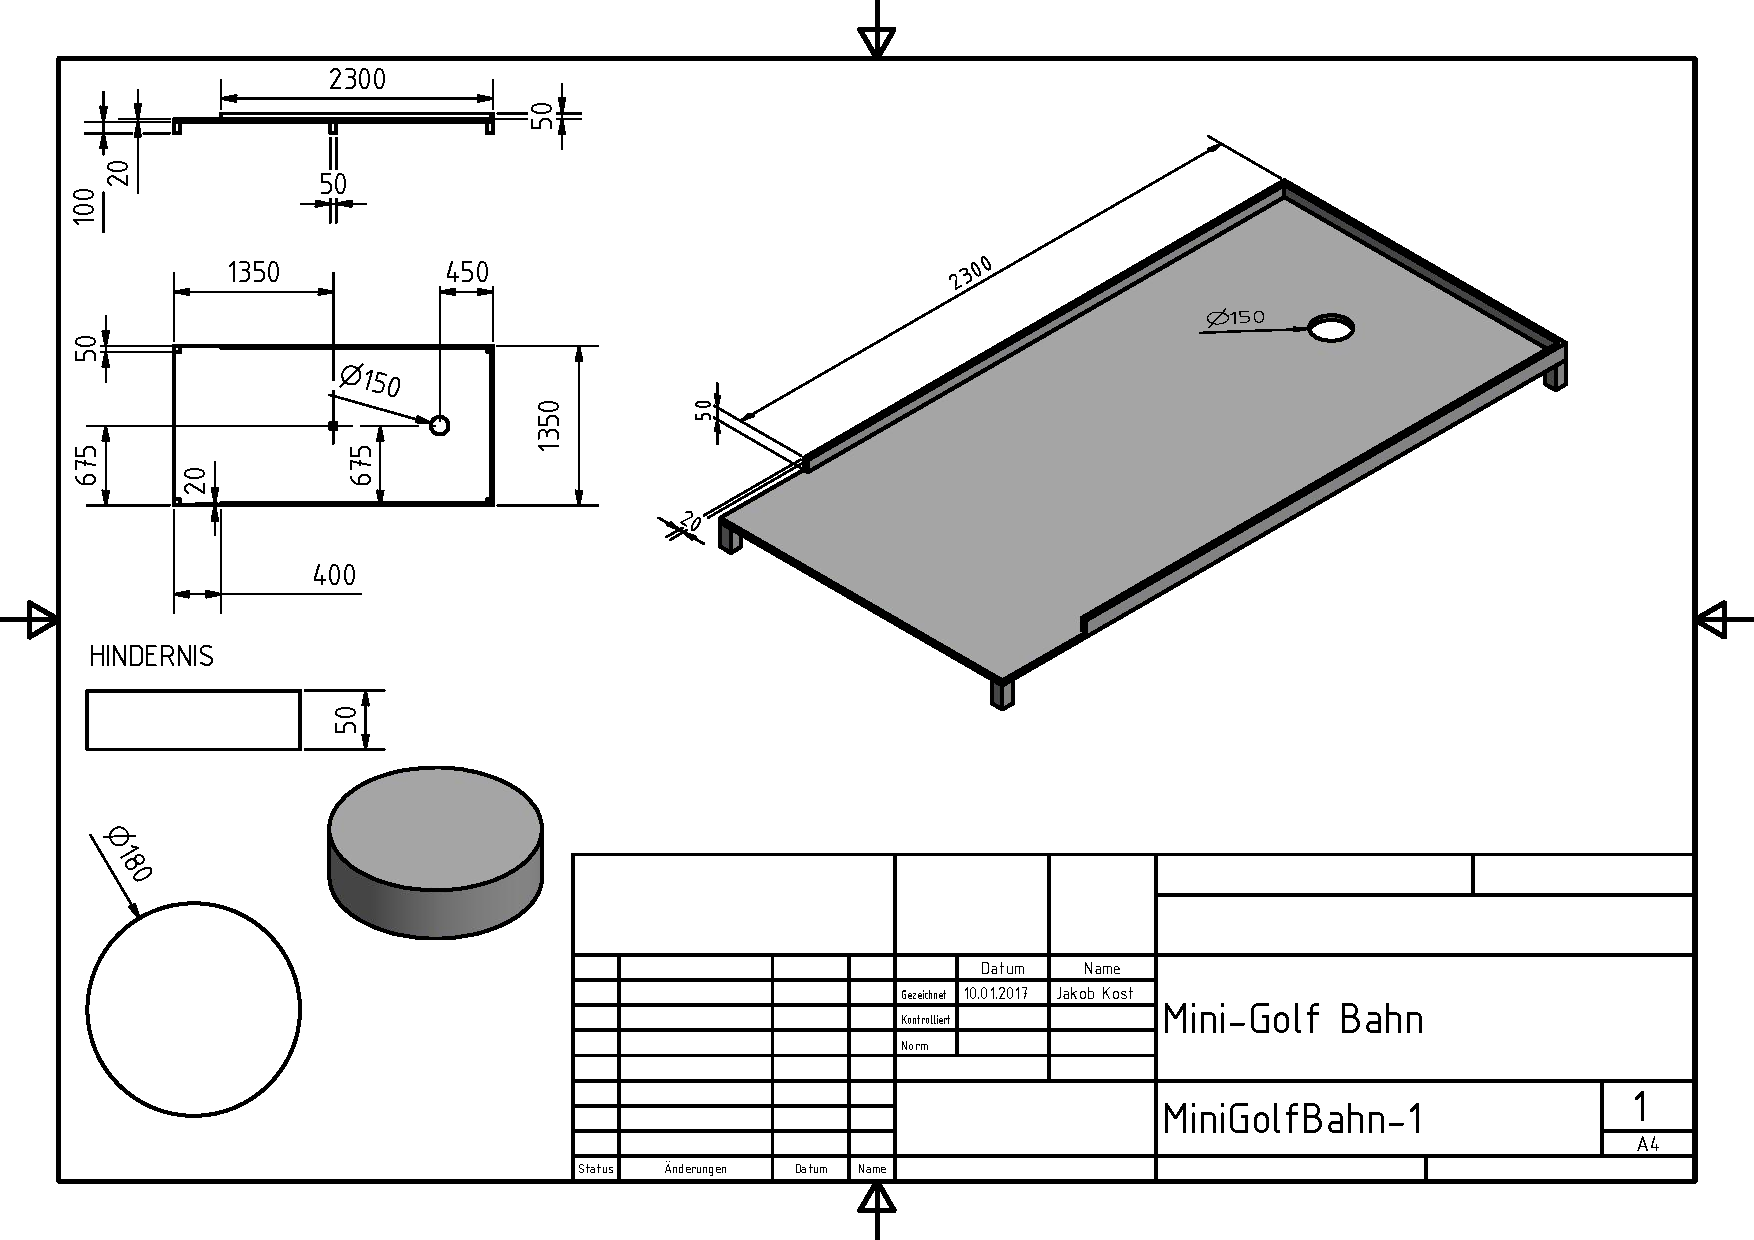
\includepdf[pages=1,pagecommand=\subsection{Minigolfbahn }]{MiniGolfBahn.pdf} 

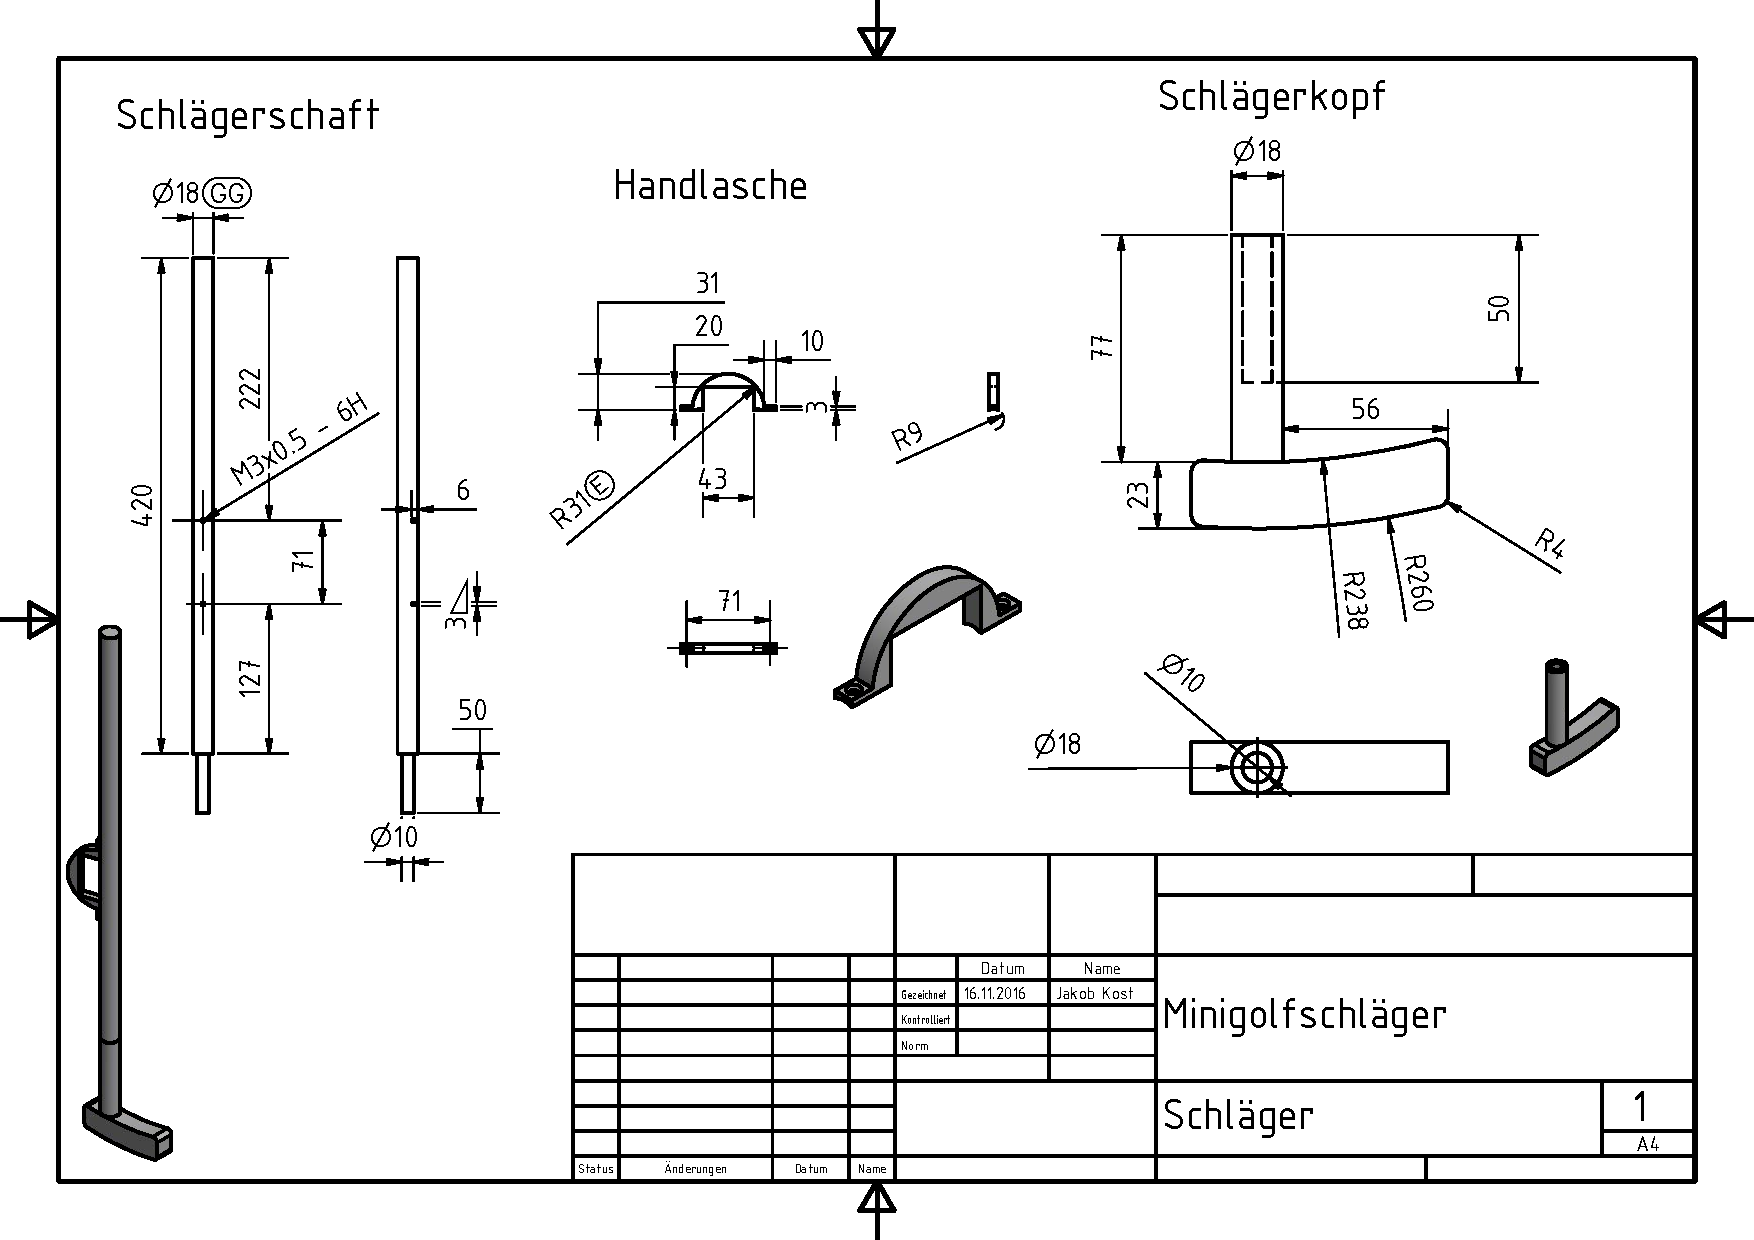
\includepdf[pages=1,pagecommand=\subsection{Schläger }]{Schlaeger.pdf} 
 

\end{document}
